\documentclass{article}
\usepackage{graphicx}
\usepackage{float}
\usepackage{caption}
\usepackage{subfigure}
\usepackage{amsmath}

\title{\textbf{TP3: Optical time domain reflectometry (OTDR)}}
\author{ HE Puyuan, ZHOU nan }
\date{ }

\begin{document}
	\maketitle
	\setlength{\parindent}{0pt} % 取消开头空格
	\section{Preparatory Questions}
	\textbf{P1}. For a fiber NA = 0.12, $\phi_c=9\mu m$, and when the optical wavelength is $\lambda=1550nm$. We can know 
	$$V = \frac{3.14}{1550}\times 10^{9}\times 9 \times 10^{-6}\times 0.12=2.188 < 2.405
	$$
	So the fiber is a single mode fiber.
	
	\textbf{P2}. The delay between the pulse emission and the reception of the reflected pulse on a default located at 10m, 1km, 10km is:
	$$t_{10m} = 6.67\times10^{-9}s, \quad t_{1km} = 6.67\times10^{-7}s, \quad t_{10km} = 6.67\times10^{-6}s$$
	
	\textbf{P3}. According to the figure
	\begin{figure}[H]
		\centering
		\includegraphics[width=0.7\linewidth]{"figure 6"}
		\caption{}
		\label{fig:figure-6}
	\end{figure}
	We can see briefly that the slope of the linear part is around 0.2. So we can know the attenuation factor is approximatedly 0.2dB/km.

	\textbf{P4}. If we want to study the noise, we should only consider the linear part in the figure 1. So the maximum distance is 25km.
	
	\textbf{P5}. If we want the power is divided by 2, by 4, the loss should be 3dB, 6dB. Considering the attenuation is 0.2dB/km, the length of the fiber should be 15km, 30km.
	
	\textbf{P6}. We can write the relation between the $\alpha_{dB} and \alpha$.
	$$\alpha_{dB}=10log_{10} \frac{1}{e^{-\alpha}}, \quad so \  \alpha=ln(10^{\frac{\alpha_{dB}}{10}})$$
	When $\alpha_{dB}=0.14dB/km$, $\alpha = ln(10^{\frac{0.14}{10}}) = 0.03224km^{-1}$.
	
	\textbf{P7}. $S = \frac{1}{m} (\frac{NA}{n})^2 = \frac{1}{4.55} (\frac{0.12}{1.4645})^2 = 0.00148$.
	
	\textbf{P8}. If we take $\alpha_s = 0.032km^{-1}$, $\tau = 1\mu s$ and $\lambda = 1550nm$, we can calculate the backscattering coefficient:
	$$R_{BS} = S \cdot \frac{\alpha_s}{2}\cdot v_g\tau = 0.00148 \times \frac{0.032}{2}\times \frac{3\times 10^5}{1.4645}\times 1\times 10^{-6}=4.85 \times 10^{-6}$$.
	
	\textbf{P9}. At the entrance of the fiber, the z = 0. If we take the input power is 12mW and the duration is $1\mu s$, we can calculate the maximum backscattering power
	$$P = R_{BS} \times P_{in} = 58.2 \times 10^{-9}W$$
	
	\section{Measurements}
	The experimental system is showed as figure 1. In our experiment, we mainly use this structure to do some measurements, according to which we study some components characterization.
	
	\begin{figure}[H]
		\centering
		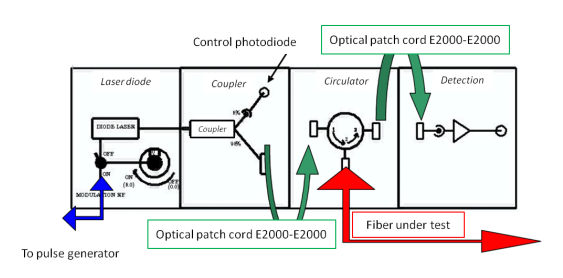
\includegraphics[width=0.7\linewidth]{figure1}
		\caption{}
		\label{fig:figure1}
	\end{figure}
	
	\subsection{Laser diode}
	In this part, we'll use part of the structure above to study the characterization of Laser diode. We take off the modulation, open the Amplifier supply, Laser diode ILX power supply and set the temperature around 20 degree. Then we connect the 95\% output to the power meter adjusted at 1550nm. Through changing the current from 0 to 100mA, we can get the results of the laser diode's power.
	
	\begin{figure}[H]
		\centering
		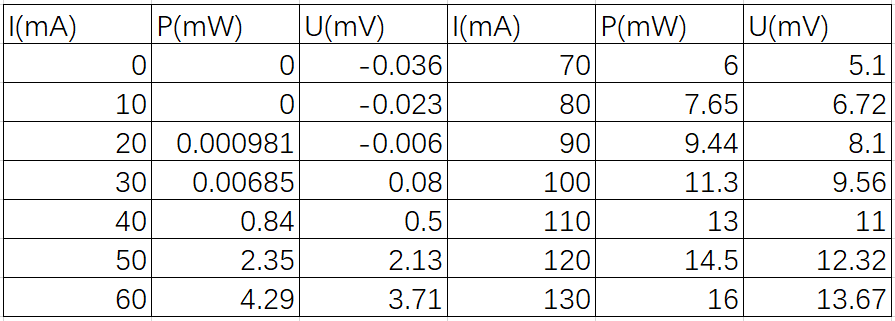
\includegraphics[width=0.7\linewidth]{table1}
		\caption{}
		\label{fig:table1}
	\end{figure}
	
	According to the data, we can draw the figure as below. And throug the figure we can briefly get the linear formula $P:f(I_{LD}) = 0.1767I_{LD} - 6.4152$ (the unit is mW and mA). Therefore, we can easily know the threshold of the laser diode is: 36.3mA. 
		
	\begin{figure}[H]
		\centering
		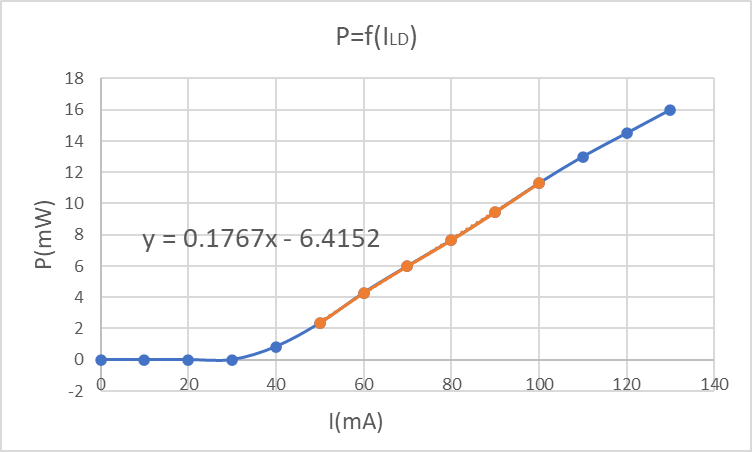
\includegraphics[width=0.7\linewidth]{figrue2}
		\caption{}
		\label{fig:figrue2}
	\end{figure}

	At the same time, we also connect the 5\% output to a photodetection, through which we can observe the voltage. The data is also noted in the table 1. we can see it in the third row and sixth row. We can focus on the situation when the current of the laser diode is 100mA. Under this circumstance the power measured by power meter is 11.3mW and the voltage read from photodetection is 9.56mV. Because this is the power from the 95\% output. Therefore the power from the 5\% output is 0.595mW. We can get the calibration of the control photodiode is 16.07V/W.
	
	\subsection{Circulator}
	In this part we want to study the circulator. We are especially interested in the connection situation between different ports of the circulator. So we firstly set the $I_{LD} = 60mA$ and measure the power of the 95\% output, finding it's 4.29mW. Then we connect this port to port number 1 of the circulator, measuring the output power of the port number 2 and number 3 separately. We find the power of port 2 is 3.10mW and the power of port 3 is 400nW. Then we connect the 95\% output to the port number 2 of the circular, measuring the output power of the port number 1 and number 3 separately. We find the power of port 1 is 30nW and the power of port 3 is 2.87mW.
	
	So we can conclude that the function of circulator. It can translate optics from port 1 to port 2 and port 2 to port 3. But the opposite direction is almost impossible. And it also can't transport light from pot 1 to port 3. The attenuation for these two situation is very large.
	
	We can also calculate the losses in the circulator between port number 1 and 2, the losses in the circulator between port number 2 and 3.
	\begin{align*}
		L_{1to2} = 10*lg(\frac{4.29}{3.10})=1.41dB \\
		L_{2to3} = 10*lg(\frac{4.29}{2.87})=1.75dB
	\end{align*}

	\subsection{OTDR detection}
	In this part, we want to study the characteristic of the detector. Below is the structure of the detector.
	\begin{figure} [H]
		\centering
		\includegraphics[width=0.7\linewidth]{"figure 3"}
		\caption{}
		\label{fig:figure-3}
	\end{figure}
	Here we set a very low current $I_P = 31.66mA$ in the laser diode, which means the power of the light is $P = 9.40 \nu W $ (below the threshold) and connect the 95\% output to the detection system by a fiber. Then we connect the output to Lecroy oscilloscope, measuring the offset voltage and saturation voltage.
	\begin{align*}
		&V_{offset}  = 940 mV,  \\
		&V_{saturation} = 1.442V 
	\end{align*}
	Therefore, we can calculate the response of the detector is:
	\begin{align*}
	G = \frac{1.442}{9.4} \times 1000 kV/W = 153.4 kV/W
	\end{align*}
	
	\section{Time resolved reflectometry}
	In this part we do a little change.  We let connect the 95\% output to the port number 1 of the circulator. And then connect the port number 2 to a 10km fiber. We detect the signal out from port number 3. 
	We also decrease the intensity of the laser to 0, switching on the pulse generator. We switch on the modulation and turn the knob at the maximum.
	
	There is a problem
	Because we've already known that for the circulator, the loss between port 1 and port 2 is 1.41dB.
	
	
	Then we modify the pulse period to find the minimum period that enable a correct measurement. We find that the period should follow the requirement
	$$T > = 98.21\mu s$$
	Through the measurement we can also measure the length of the fiber.
	\begin{figure} [H]
		\centering
		\includegraphics[width=0.7\linewidth]{"figure 4"}
		\caption{}
		\label{fig:figure-4}
	\end{figure}
	We can see the duration of the linear region in the figure is 87.676 us. So we can calculate the length of the fiber
	$$L = \frac{3\times 10^8}{1.4645} \times 87.6767 \times 10^{-6}\times \frac{1}{2}m = 8.98 km$$
	Because the voltage is linear to the power of the light. We can directly use the voltage to calculate the attenuation of the fiber. Through the oscilloscope we  measure the maximum voltage is $U_{max} = 32.8mV$, the minimum voltage is $U_{max} = 14.8mV$. So the loss is 
	\begin{align*}
		\alpha = 10 lg\frac{14.8}{32.8} \times \frac{1}{8.98} = 3.8dB/km
	\end{align*}
	From what I've mentioned above, we know that the maximum detected voltage is 32.8mV. Because the photodetector's response is 120kV/W. So the light out from port 3 of the circulator is 0.2733uW. So the beginning of the fiber's backscattered power at port 2 is $0.2733\mu W \times \frac{4.29}{2.87} = 0.409\mu W$.
	
	Considering $S = \frac{1}{m}(\frac{NA}{n})^2 = \frac{1}{4}(\frac{0.12}{1.4645})^2 = 0.00168, \quad \tau = 12.40\mu s , \quad \alpha_S = 0.032km^{-1}$, we can calculate that 
	\begin{align*}
		R_{BS} = S\cdot \frac{\alpha_S}{2}\cdot v_g \tau  = 0.00168 \times \frac{0.032}{2} \frac{3*10^5}{1.4645}\times 12.4\times 10^{-6} = 68.3\times 10^{-6}.
	\end{align*}

	In fact in order to calculate the loss of the fiber , we needn't to know the value of the R. We know that the optical power of the backscattering is linear to the value of R. And it's also linear to the voltage of the detector. When we calculate the loss, we do the division. All the coefficient will be eliminate. So they won't infect our calculation result.
	
	Then we want to measure the backscattered power at the beginning of the fiber for different pulse duration from 0 to 5 $\mu s$. We note the results in the following table.
	
	\begin{figure}[H]
		\centering
		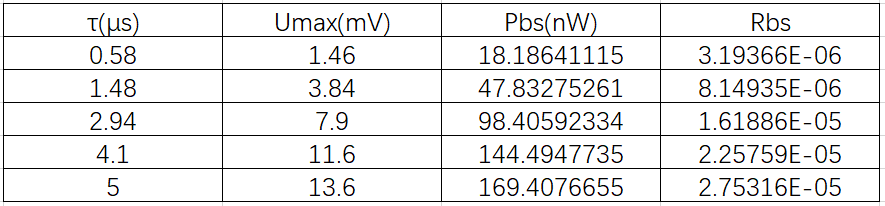
\includegraphics[width=0.7\linewidth]{table2}
		\caption{}
		\label{fig:table2}
	\end{figure}

	Because We already the response of the detector, we can easily calculate the power according to the voltage. Then considering the loss between port 2 and port 3, we can get the backscarttered optical power as we present in the table. Also for different value of $\tau$, according to the formula of $R_{BS}$ I presented above, we can calculate the value of $R_{BS}$. I also present the values in the table.
	
	Also according to our analysis, the shorter the pulse, the more accurate measurement can be achieved. When the pulse time is too long, we cannot accurately obtain the backscattered signal at a certain time, because the signals emitted during a single pulse time will interfere with each other. At this time, it is difficult for us to analyze the length of the optical fiber, and related parameters such as loss.
	
	(Above the results about the loss of the fiber and the length of the fiber may noy be correct. Because the connect of the 10km fiber doesn't work well. That's also why we don't use it in the following steps.)
	\\
	Then we connect a 5km fiber with a 15km fiber, to study the OTDR signal. Because the lab doesn't provide the Matlab, we can't do the analysis. We just get the result in oscilloscope.
	
	\begin{figure}[H]
		\centering
		\includegraphics[width=0.7\linewidth]{"figure 5"}
		\caption{}
		\label{fig:figure-5}
	\end{figure}
	
	Here we can clearly see the separate point, according to which we can calculate the length of the two fiber. We wiil also be able to study the attenuation factor for the two fibers.


\end{document}